
%%%%%%%%%%%%%%%%%%%% 附录 %%%%%%%%%%%%%%%%%%%%%

% 添加附录, 如不需要可以把附录部分注释
\appendix

% 附录正文
\chapter{这是第一个附录}

\section{附录A的小节}

这里是附录环境\index{附录环境}.

附录公式及编号
\begin{equation}\label{eq:abc}
  a^2+b^2=c^2.
\end{equation}

附录的图片: 如图~\ref{fig:sinx2}.
\begin{figure}[htp!]
  \centering
  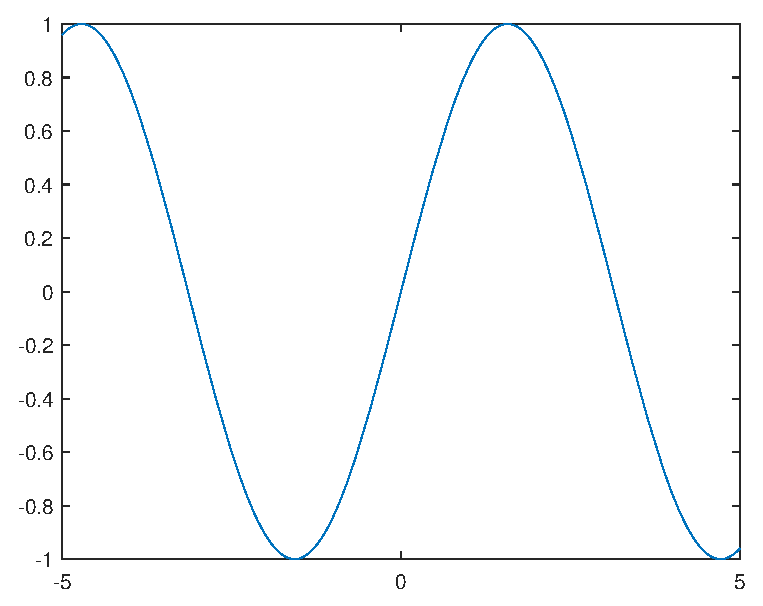
\includegraphics[width=0.45\linewidth]{image1.eps}
  \caption{函数 $y=\sin(x)$ 的图像}\label{fig:sinx2}
\end{figure}


附录的表格: 表~\ref{tab:heightweight2}.

\begin{table}[htp!]
\centering
% PLCR已经定义
\caption{某校学生身高体重样本}
\label{tab:heightweight2}
\begin{tabularx}{0.9\textwidth}{P{1.5cm}CCC}
\toprule
序号 & 年龄 & 身高 & 体重 \\
\midrule
001 & 15 & 156 & 42 \\
002 & 16 & 158 & 45 \\
003 & 14 & 162 & 48 \\
004 & 15 & 163 & 50 \\
\cmidrule{2-4}
平均 & 15 & 159.75 & 46.25 \\
\bottomrule
\end{tabularx}
\end{table}


\chapter{这是第二个附录}

\section{附录B的小节}

这里是附录环境.

附录内容附录内容附录内容内容附录内容附录内容附录内容附录内容附录内容附录内容附录内容附录内容附录内容附录内容附录内容附录内容附录内容附录内容附录内容附录内容附录内容正文内容正文.内容附录内容附录内容附录内容附录内容附录内容附录内容附录内容附录内容附录内容附录内容附录内容附录内容附录内容附录内容附录内容附录内容附录内容文内容正文内容.
